\section{Experiments}
\label{sec:experiments}

\subsection{Current Evidence}

We first summarize the current downstream checkpoint sweep that motivated this paper.
The non-meta baseline is the improved SpiderMark verifier, and the meta-learning result uses the downstream meta checkpoint selected by validation accuracy at epoch 116.
Both rows are computed from the repository's attack-evaluation summaries; the exact artifact paths are recorded in the experiment notes rather than printed in the main text.
Table~\ref{tab:stage1_generated_meta_vs_nometa} reports accuracy and AUROC under nine transformations.

% Auto-generated by scripts/stage1_aggregate_benchmark.ps1
\begin{table*}[t]
\centering
\caption{Stage 1 comparison between non-meta SpiderMark and the selected MetaSpiderMark verifier.}
\label{tab:stage1_generated_meta_vs_nometa}
\resizebox{\textwidth}{!}{
\begin{tabular}{lrrrrrr}
\toprule
\textbf{Attack} & \textbf{No-meta Acc} & \textbf{No-meta AUROC} & \textbf{Meta Acc} & \textbf{Meta AUROC} & \textbf{$\Delta$ Acc} & \textbf{$\Delta$ AUROC} \\
\midrule
clean & 0.9467 & 0.9904 & 0.9800 & 0.9995 & +0.0333 & +0.0091 \\
jpeg\_strong & 0.8720 & 0.9409 & 0.9347 & 0.9867 & +0.0627 & +0.0457 \\
msg\_app\_combo & 0.6813 & 0.8468 & 0.9173 & 0.9558 & +0.2360 & +0.1090 \\
down\_up & 0.9133 & 0.9713 & 0.9533 & 0.9939 & +0.0400 & +0.0226 \\
blur & 0.8160 & 0.8757 & 0.9040 & 0.9678 & +0.0880 & +0.0920 \\
random\_crop & 0.8787 & 0.9503 & 0.9027 & 0.9691 & +0.0240 & +0.0188 \\
occlusion & 0.9573 & 0.9878 & 0.9800 & 0.9993 & +0.0227 & +0.0114 \\
geom\_warp & 0.8560 & 0.9381 & 0.8893 & 0.9626 & +0.0333 & +0.0245 \\
train\_aug\_mix & 0.7280 & 0.8620 & 0.8027 & 0.8830 & +0.0747 & +0.0211 \\
\midrule
\textbf{Mean} & \textbf{0.8499} & \textbf{0.9293} & \textbf{0.9182} & \textbf{0.9686} & \textbf{+0.0683} & \textbf{+0.0394} \\
\bottomrule
\end{tabular}
}
\end{table*}


The meta-learned verifier improves accuracy on every listed attack.
The largest gain is on \texttt{msg\_app\_combo}, a compound transformation intended to emulate common messaging-app degradation.
This suggests that episodic exposure to downstream tasks can improve verifier stability under transformations that are difficult for a static supervised verifier.

\subsection{Meta-Training Diagnostics}

The current repository also contains diagnostics from a 2000-step meta-training run over seven candidate attack tasks: clean, down-up sampling, crop, JPEG, blur, message-app processing, and occlusion.
These artifacts are not yet treated as final scheduler benchmark evidence, but they are useful for understanding the training dynamics and for deciding what to benchmark next.
Figure~\ref{fig:training_diagnostics} summarizes the meta-loss trajectory, sampled task distribution, and residual task-weight corrections proposed by the LLM scheduler.

\begin{figure*}[t]
    \centering
    \begin{subfigure}[t]{0.32\textwidth}
        \centering
        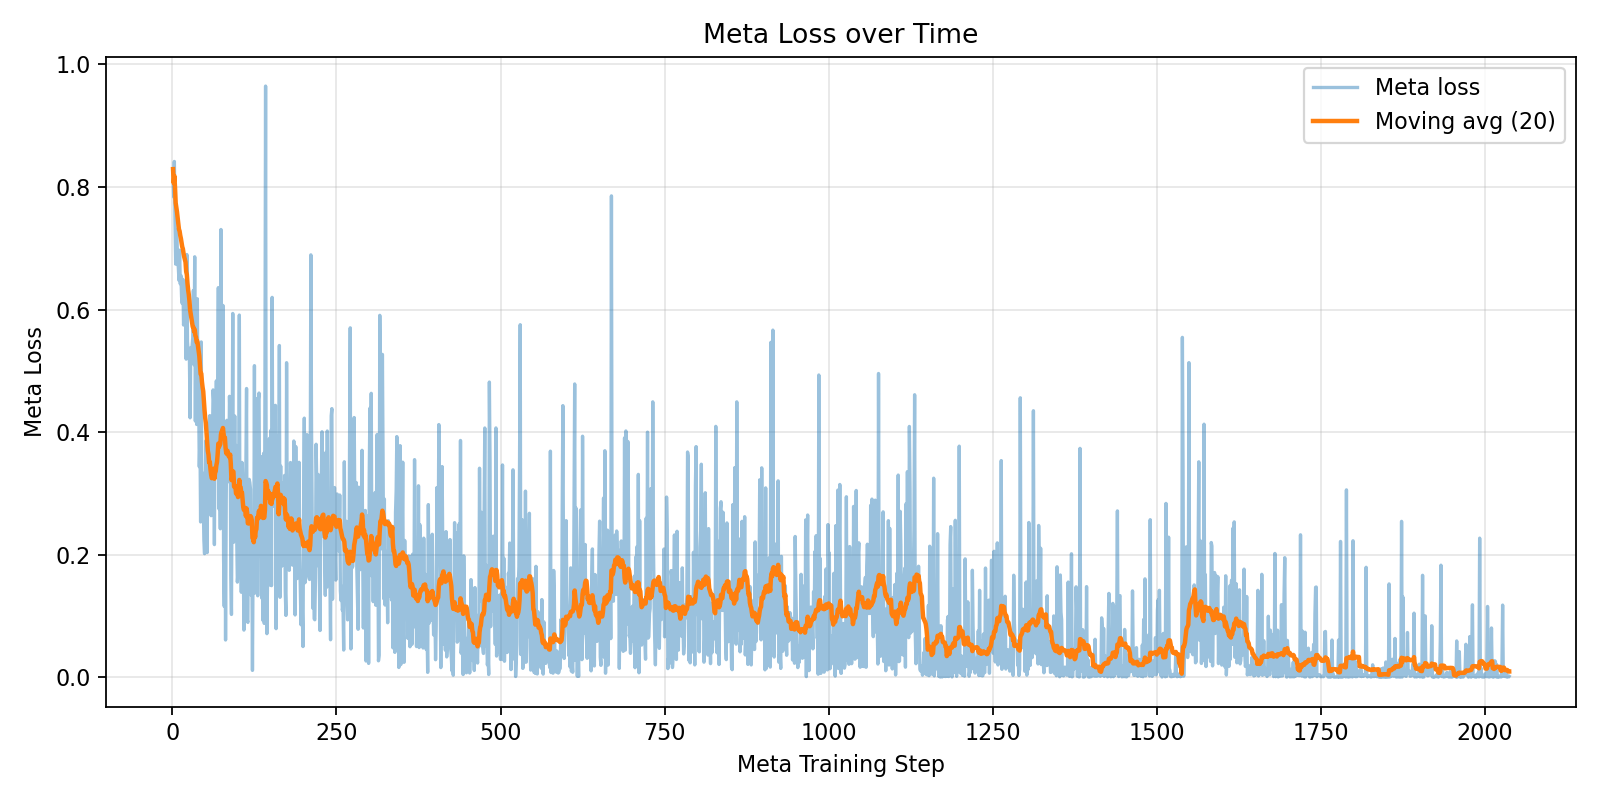
\includegraphics[width=\linewidth]{figures/meta_loss_curve.png}
        \caption{Meta-loss curve}
    \end{subfigure}
    \hfill
    \begin{subfigure}[t]{0.32\textwidth}
        \centering
        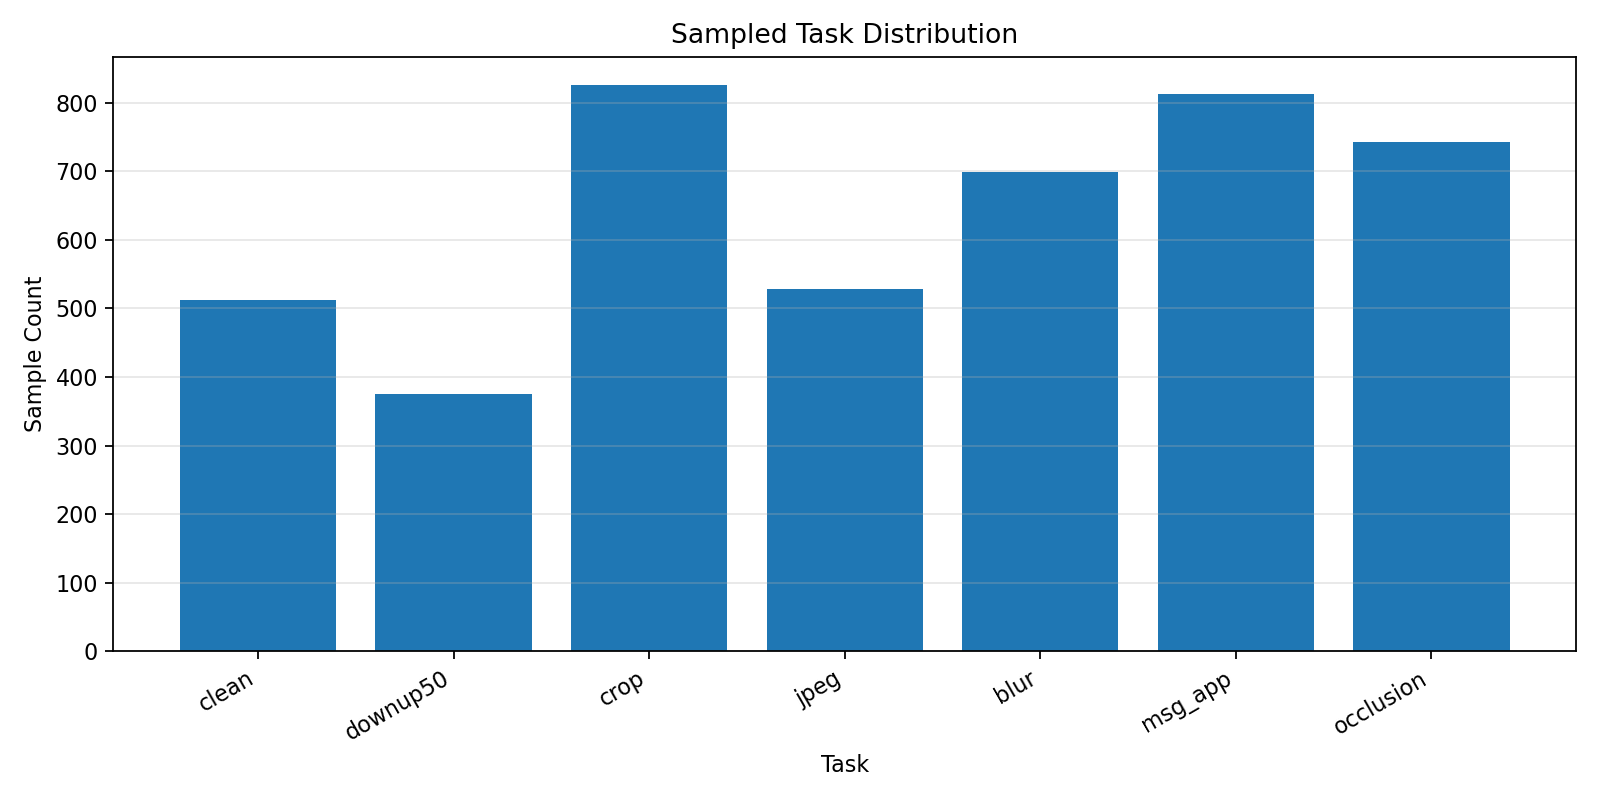
\includegraphics[width=\linewidth]{figures/sampled_task_distribution.png}
        \caption{Sampled tasks}
    \end{subfigure}
    \hfill
    \begin{subfigure}[t]{0.32\textwidth}
        \centering
        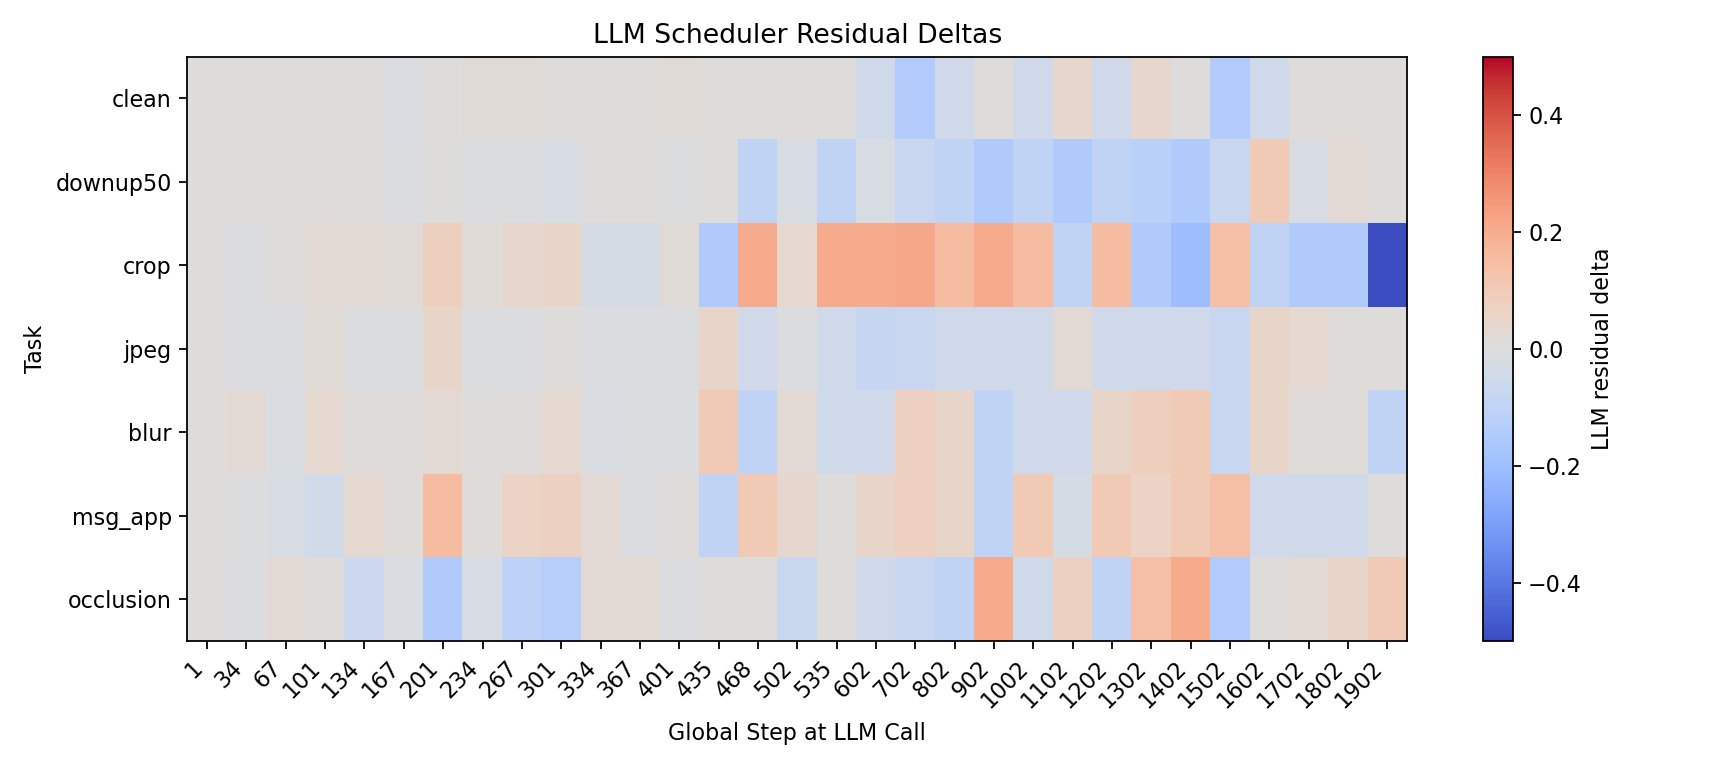
\includegraphics[width=\linewidth]{figures/llm_delta_heatmap.png}
        \caption{LLM residual deltas}
    \end{subfigure}
    \caption{\textbf{Available meta-training diagnostics.}
    These plots show that the current implementation logs optimization behavior, task exposure, and scheduler corrections during meta-training.
    They should be used as diagnostic evidence and sanity checks; the final paper still requires controlled scheduler baselines under matched compute budgets.}
    \label{fig:training_diagnostics}
\end{figure*}

\subsection{Available Proposed-Method Checkpoint}

In addition to the validation-selected checkpoint in Table~\ref{tab:stage1_generated_meta_vs_nometa}, the current notebook sweep evaluates the final 2000-step downstream meta checkpoint.
This checkpoint is useful as the proposed-method row for the scheduler benchmark because it is already evaluated on the same nine downstream attacks.
Table~\ref{tab:current_final_checkpoint_summary} summarizes the final-checkpoint aggregate numbers from the notebook artifact.

\begin{table}[t]
\centering
\small
\caption{Current final-checkpoint downstream robustness from the checkpoint-sweep notebook.}
\label{tab:current_final_checkpoint_summary}
\begin{tabular}{lcc}
\toprule
\textbf{Metric} & \textbf{Mean} & \textbf{Worst attack} \\
\midrule
Accuracy & 0.8959 & 0.7480 \\
AUROC & 0.9545 & 0.8389 \\
\bottomrule
\end{tabular}
\end{table}

\subsection{Benchmark Design}

The final evaluation is organized around two complementary questions.
First, does episodic verifier training improve SpiderMark robustness over a non-meta verifier?
Second, under matched verifier architecture, attack pool, support/query sizes, and 2000-step training budget, which task scheduler provides the strongest downstream robustness?
Uniform sampling serves as a minimal anchor, while cyclic scheduling is kept as an optional diagnostic rather than a main compute target.
The scheduler benchmark compares non-contextual UCB bandits, ATS-style adaptive task scheduling, BASS-style contextual bandits, and ASR-style adaptive sampling.
A GCP-style task-weighting proxy is included as an appendix candidate because its original class-combination setting does not map exactly to our attack-task pool.
DERTS remains an important future baseline, but a faithful implementation requires full task-pool gradient subset optimization rather than the scalar online feedback currently available in the training loop.

\begin{table*}[t]
\centering
\small
\caption{Planned scheduler benchmark table. Blank cells denote runs that are not yet trained and evaluated under the matched 2000-step budget. The proposed-method row uses the already available final-checkpoint notebook evaluation.}
\label{tab:scheduler_benchmark_skeleton}
\resizebox{\textwidth}{!}{
\begin{tabular}{llcccccc}
\toprule
\textbf{Method} & \textbf{Scheduler family} & \textbf{Mean Acc.} & \textbf{Worst Acc.} & \textbf{Mean AUROC} & \textbf{Worst AUROC} & \textbf{Train steps} & \textbf{Status} \\
\midrule
Uniform & random anchor &  &  &  &  & 2000 & checkpoint ready, eval pending \\
Bandit-UCB & non-contextual bandit &  &  &  &  & 2000 & training \\
ATS-style~\cite{yao2021ats} & adaptive task scheduler &  &  &  &  & 2000 & queued \\
BASS-style~\cite{ban2023bass} & contextual neural bandit principle &  &  &  &  & 2000 & queued \\
ASR-style & diversity/entropy/difficulty sampler &  &  &  &  & 2000 & queued \\
GCP-style proxy & exponential task weighting &  &  &  &  & 2000 & optional appendix \\
\textbf{MetaSpiderMark} & proposed verifier training & \textbf{0.8959} & \textbf{0.7480} & \textbf{0.9545} & \textbf{0.8389} & 2000 & evaluated \\
\bottomrule
\end{tabular}
}
\end{table*}

\subsection{Planned Metrics}

We will report accuracy at a fixed operating threshold, AUROC, and where possible threshold stability across attacks.
Because watermark verification is often deployed at a single threshold, accuracy under a fixed policy is important even when AUROC is high.
For image quality and semantic preservation, the benchmark should reuse the SpiderMark metrics: FID and CLIP image-text similarity.
Because the watermark injection mechanism is unchanged, these quality metrics are supporting evidence rather than the main comparison axis.
For meta-learning itself, we should additionally report training cost, checkpoint sensitivity, task sampling distribution, and performance variance across random seeds.

\subsection{Experiment Roadmap}

The current table is promising but not yet sufficient for a CVPR submission.
We organize the remaining experiments around a SOTA/canonical meta-learning comparison plus a scheduler ablation.
The repository-level execution plan is maintained in \texttt{BENCHMARK\_PLAN.md}; here we summarize the benchmark structure expected in the final paper.

\paragraph{Stage 1: anchor baselines.}
This stage establishes the fixed reference points: the improved non-meta SpiderMark verifier and the currently available meta-trained verifier checkpoints.
It answers whether the direction is worth expanding and provides the non-meta anchor for all later scheduler deltas.

\paragraph{Stage 2: scheduler benchmark.}
This stage trains and evaluates the fixed comparison set in Table~\ref{tab:scheduler_benchmark_skeleton}.
The current execution plan is training-first: finish all selected scheduler checkpoints, then run the same downstream evaluation suite for every row.
This avoids mixing preliminary eval settings with final matched-compute results.

\paragraph{Stage 3: SOTA/canonical meta-learning comparison.}
After the scheduler comparison is stable, this stage fixes the scheduler and compares FOMAML, MAML, ANIL, Reptile, Matching Networks-style attention, Prototypical Networks-style prototypes, and an R2D2-style differentiable ridge solver head under the same attack pool, number of meta-training steps, support/query sizes, and checkpoint-selection rule.
This separates improvements from the meta-learning update itself from improvements caused by task scheduling.

\paragraph{Stage 4: stability and ablations.}
This stage checks that the scheduler ranking is stable rather than a single-run artifact.
It should include seed variance, checkpoint selection, held-out attacks or held-out prompts, scheduler overhead, and quality metrics for the final selected configuration.
External watermarking baselines can be included as contextual comparisons, but they are not the main benchmark required to support the paper's claim.

The concrete missing items are:
\begin{itemize}
    \item repeat the meta versus no-meta comparison across multiple seeds;
    \item finish the seed-0 scheduler benchmark for UCB, ATS-style, BASS-style, and ASR-style task sampling;
    \item optionally evaluate the GCP-style proxy as an appendix scheduler row;
    \item evaluate FOMAML, MAML, ANIL, Reptile, Matching Networks-style, Prototypical Networks-style, and R2D2-style ridge baselines under the selected fixed scheduler and compute budget;
    \item compare checkpoint-selection strategies across the full downstream sweep;
    \item test transfer to an unseen prompt or dataset split, ideally COCO as in the SpiderMark paper;
    \item measure scheduler overhead, image quality, and semantic preservation for the final selected method.
\end{itemize}
